\section{SuperCon3D}
{{\footnotesize
\begin{description}[labelwidth=5em, labelsep=1em, leftmargin=*, align=left, itemsep=0.3em, parsep=0em]
  \item[date:] 2024-12-13
  \item[version:] TODO
  \item[last\_updated:] 2024-12
  \item[expired:] unknown
  \item[valid:] yes
  \item[valid\_date:] TODO
  \item[url:] \href{https://neurips.cc/virtual/2024/poster/97553}{https://neurips.cc/virtual/2024/poster/97553}
  \item[doi:] TODO
  \item[domain:] Materials Science; Superconductivity
  \item[focus:] Dataset and models for predicting and generating high-Tc superconductors using 3D crystal structures
  \item[keywords:]
    - superconductivity
    - crystal structures
    - equivariant GNN
    - generative models
  \item[summary:] SuperCon3D introduces 3D crystal structures with associated critical temperatures (Tc) and two deep-learning models: SODNet (equivariant graph model) and DiffCSP-SC (diffusion generator) designed to screen and synthesize high-Tc candidates :contentReference[oaicite:3]\{index=3\}.

  \item[licensing:] TODO
  \item[task\_types:]
    - Regression (Tc prediction)
    - Generative modeling
  \item[ai\_capability\_measured:]
    - Structure-to-property prediction
    - structure generation
  \item[metrics:]
    - MAE (Tc)
    - Validity of generated structures
  \item[models:]
    - SODNet
    - DiffCSP-SC
  \item[ml\_motif:]
    - Materials Modeling
  \item[type:] Dataset + Models
  \item[ml\_task:]
    - Regression, Generation
  \item[solutions:] TODO
  \item[notes:] Demonstrates advantage of combining ordered and disordered structural data in model design :contentReference[oaicite:4]\{index=4\}.

  \item[contact.name:] Zhong Zuo
  \item[contact.email:] unknown
  \item[results.links.name:] ChatGPT LLM
  \item[fair.reproducible:] Yes
  \item[fair.benchmark\_ready:] Yes
  \item[ratings.software.rating:] 0
  \item[ratings.software.reason:] Not analyzed.

  \item[ratings.specification.rating:] 10.0
  \item[ratings.specification.reason:] Multimodal task (segmentation + natural language QA pairs);.

  \item[ratings.dataset.rating:] 10.0
  \item[ratings.dataset.reason:] sonar imagery + masks + descriptions, georeferenced and labeled with QA

  \item[ratings.metrics.rating:] 9.0
  \item[ratings.metrics.reason:] Pixel accuracy and QA metrics clearly defined; tasks split by modality.

  \item[ratings.reference\_solution.rating:] 8.0
  \item[ratings.reference\_solution.reason:] Baseline models (SegFormer, ViLT) are cited, partial configs likely available.

  \item[ratings.documentation.rating:] 8.5
  \item[ratings.documentation.reason:] Paper + GitHub metadata and processing details are comprehensive, though full dataset is not yet available.

  \item[id:] supercond
  \item[Citations:] \cite{neurips2024_c4e3b55e}
  \item[Ratings:]
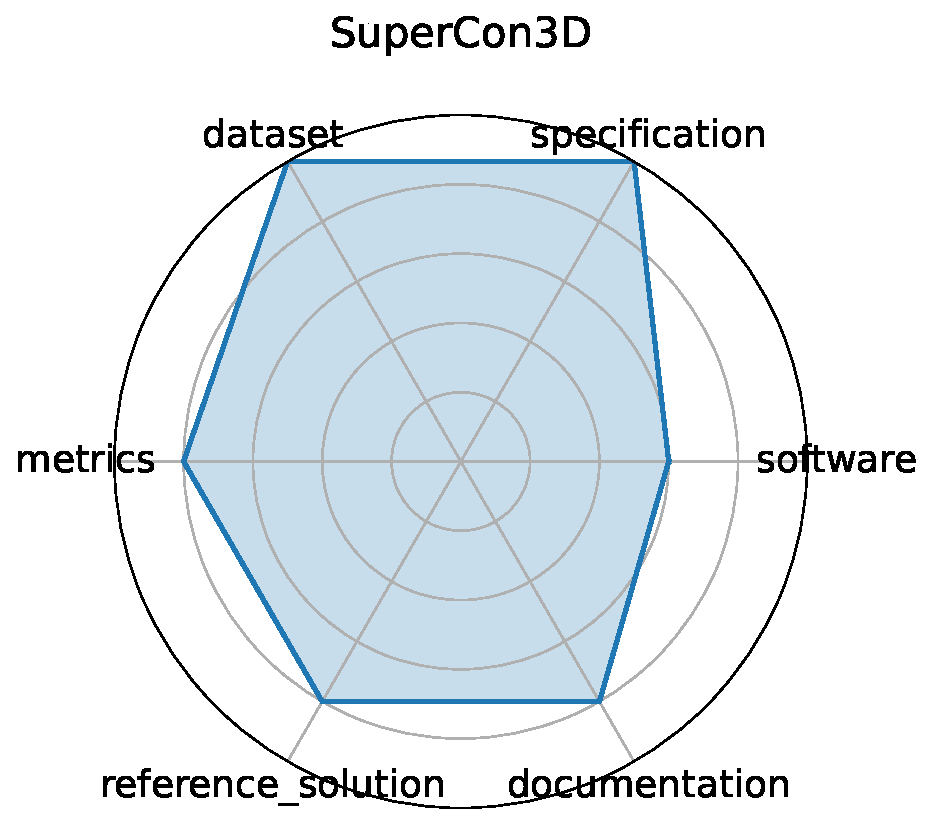
\includegraphics[width=0.2\textwidth]{supercond_radar.pdf}
\end{description}
}}
\clearpage